\documentclass{article}
\usepackage[utf8]{inputenc}
\usepackage{amsmath,amsthm,amssymb,marvosym,mathrsfs,amsfonts,amscd, mathtools}
\usepackage[margin=2.5cm,headsep=0.5cm]{geometry}

% Hyperlink shit
\usepackage{hyperref}
\hypersetup{
    colorlinks,
    citecolor=black,
    filecolor=black,
    linkcolor=black,
    urlcolor=black
}

% Colors
\usepackage{xcolor}

% Clean SI Units
\usepackage{siunitx}

% Itemize shit
\usepackage{enumitem}

% Bra ket notation
\usepackage{braket}

% Cancel things out in equations
\usepackage[makeroom]{cancel}

% Better support for graphics and figures
\usepackage{graphicx}
\graphicspath{{./images/}}
\usepackage{wrapfig}
\usepackage{float}

% Highlighting
\usepackage{color,soul}

% Caption figures and tables
\usepackage{caption}

\usepackage{gensymb}
\usepackage{relsize}

% Framing shit
\usepackage{mdframed}
\usepackage{framed}

% Make multiple rows in a table
\usepackage{booktabs}
\usepackage{multirow}


% Tikz Package Shit
\usepackage{pgf,tikz,pgfplots}
\usepackage{tikz-3dplot}
\pgfplotsset{compat=1.15}
\usetikzlibrary{arrows}
\usetikzlibrary{calc}
\usetikzlibrary{scopes}
\usetikzlibrary{angles, quotes}
\usetikzlibrary{svg.path}
\usetikzlibrary{arrows}
% Draw an arc from the center
\def\centerarc[#1](#2)(#3:#4:#5)% Syntax: [draw options] (center) (initial angle:final angle:radius)
    { \draw[#1] ($(#2)+({#5*cos(#3)},{#5*sin(#3)})$) arc (#3:#4:#5); }
\pgfplotsset{compat=newest}    


% Circled numbers that don't look like a shit
\newcommand*\circled[1]{\tikz[baseline=(char.base)]{
            \node[shape=circle,draw,inner sep=2pt] (char) {#1};}}


% Blackboard bold shit
\usepackage{bm}
\DeclareSymbolFont{bbold}{U}{bbold}{m}{n}
\DeclareSymbolFontAlphabet{\mathbbold}{bbold}

% Custom environments - useful for math shit
\setlength{\parindent}{0pt}
\DeclarePairedDelimiter\floor{\lfloor}{\rfloor}
\newcommand{\N}{\mathbb{N}}
\newcommand{\Z}{\mathbb{Z}}
\newcommand{\R}{\mathbb{R}}
\newcommand{\Q}{\mathbb{Q}} 
\newcommand{\I}{\mathbb{I}}
\newenvironment{theorem}[2][Theorem]{\begin{trivlist}
\item[\hskip \labelsep {\bfseries #1}\hskip \labelsep {\bfseries #2.}]}{\end{trivlist}}
\newenvironment{THEOREM}[2][Theorem]{\begin{trivlist}
\item[\hskip \labelsep {\bfseries #2}\hskip \labelsep {\bfseries #1.}]}{\end{trivlist}}
\newenvironment{lemma}[2][Lemma]{\begin{trivlist}
\item[\hskip \labelsep {\bfseries #1}\hskip \labelsep {\bfseries #2.}]}{\end{trivlist}}
\newenvironment{LEMMA}[2][Lemma]{\begin{trivlist}
\item[\hskip \labelsep {\bfseries #2}\hskip \labelsep {\bfseries #1.}]}{\end{trivlist}}
\newenvironment{exercise}[2][Exercise]{\begin{trivlist}
\item[\hskip \labelsep {\bfseries #1}\hskip \labelsep {\bfseries #2.}]}{\end{trivlist}}
\newenvironment{reflection}[2][Reflection]{\begin{trivlist}
\item[\hskip \labelsep {\bfseries #1}\hskip \labelsep {\bfseries #2.}]}{\end{trivlist}}
\newenvironment{proposition}[2][Proposition]{\begin{trivlist}
\item[\hskip \labelsep {\bfseries #1}\hskip \labelsep {\bfseries #2.}]}{\end{trivlist}}
\newenvironment{corollary}[2][Corollary]{\begin{trivlist}
\item[\hskip \labelsep {\bfseries #1}\hskip \labelsep {\bfseries #2.}]}{\end{trivlist}}
\renewcommand\qedsymbol{$\blacksquare$}

% Custom environments for this project
\newenvironment{interlude}[2][Interlude]
{\textbf{#1}: }{}

% Number equations within sections
% \numberwithin{equation}{section}

% Code listing
\usepackage{listings}
\definecolor{codegreen}{rgb}{0,0.6,0}
\definecolor{codegray}{rgb}{0.5,0.5,0.5}
\definecolor{codepurple}{rgb}{0.58,0,0.82}
\definecolor{backcolour}{rgb}{0.95,0.95,0.92}
\lstdefinestyle{mystyle}{
    backgroundcolor=\color{backcolour},   
    commentstyle=\color{codegreen},
    keywordstyle=\color{blue},
    numberstyle=\tiny\color{codegray},
    stringstyle=\color{codepurple},
    basicstyle=\footnotesize,
    breakatwhitespace=false,         
    breaklines=true,                 
    captionpos=b,                    
    keepspaces=true,                 
    numbers=left,                    
    numbersep=5pt,                  
    showspaces=false,                
    showstringspaces=false,
    showtabs=false,                  
    tabsize=2
}
\lstset{style=mystyle}

\usepackage{upgreek}

% Unit vectors
\newcommand{\ihat}{\mathbf{\hat{i}}}
\newcommand{\jhat}{\mathbf{\hat{j}}}
\newcommand{\khat}{\mathbf{\hat{k}}}
\newcommand{\ehat}{\mathbf{\hat{e}}}
\newcommand{\rhat}{\mathbf{\hat{r}}}
\newcommand{\nhat}{\mathbf{\hat{n}}}
\newcommand{\thetahat}{\boldsymbol{\hat{\uptheta}}}
\newcommand{\phihat}{\boldsymbol{\hat{\upphi}}}


% Colors
\definecolor{ao}{HTML}{6F0EED}
\definecolor{DARK_BLUE}{HTML}{236B8E}
\definecolor{DARK_BROWN}{HTML}{8B4513}
\definecolor{LIGHT_BROWN}{HTML}{CD853F}
\definecolor{BLUE_E}{HTML}{1C758A}
\definecolor{BLUE_D}{HTML}{29ABCA}
\definecolor{BLUE_C}{HTML}{58C4DD}
\definecolor{BLUE_B}{HTML}{9CDCEB}
\definecolor{BLUE_A}{HTML}{C7E9F1}
\definecolor{TEAL_E}{HTML}{49A88F}
\definecolor{TEAL_D}{HTML}{55C1A7}
\definecolor{TEAL_C}{HTML}{5CD0B3}
\definecolor{TEAL_B}{HTML}{76DDC0}
\definecolor{TEAL_A}{HTML}{ACEAD7}
\definecolor{GREEN_E}{HTML}{699C52}
\definecolor{GREEN_D}{HTML}{77B05D}
\definecolor{GREEN_C}{HTML}{83C167}
\definecolor{GREEN_B}{HTML}{A6CF8C}
\definecolor{GREEN_A}{HTML}{C9E2AE}
\definecolor{YELLOW_E}{HTML}{E8C11C}
\definecolor{YELLOW_D}{HTML}{F4D345}
\definecolor{YELLOW_C}{HTML}{FFFF00}
\definecolor{YELLOW_B}{HTML}{FFEA94}
\definecolor{YELLOW_A}{HTML}{FFF1B6}
\definecolor{GOLD_E}{HTML}{C78D46}
\definecolor{GOLD_D}{HTML}{E1A158}
\definecolor{GOLD_C}{HTML}{F0AC5F}
\definecolor{GOLD_B}{HTML}{F9B775}
\definecolor{GOLD_A}{HTML}{F7C797}
\definecolor{RED_E}{HTML}{CF5044}
\definecolor{RED_D}{HTML}{E65A4C}
\definecolor{RED_C}{HTML}{FC6255}
\definecolor{RED_B}{HTML}{FF8080}
\definecolor{RED_A}{HTML}{F7A1A3}
\definecolor{MAROON_E}{HTML}{94424F}
\definecolor{MAROON_D}{HTML}{A24D61}
\definecolor{MAROON_C}{HTML}{C55F73}
\definecolor{MAROON_B}{HTML}{EC92AB}
\definecolor{MAROON_A}{HTML}{ECABC1}
\definecolor{PURPLE_E}{HTML}{644172}
\definecolor{PURPLE_E}{HTML}{715582}
\definecolor{PURPLE_E}{HTML}{9A72AC}
\definecolor{PURPLE_E}{HTML}{B189C6}
\definecolor{PURPLE_E}{HTML}{CAA3E8}
\definecolor{WHITE}{HTML}{FFFFFF}
\definecolor{BLACK}{HTML}{000000}
\definecolor{LIGHT_GRAY}{HTML}{BBBBBB}
\definecolor{GRAY}{HTML}{888888}
\definecolor{DARK_GRAY}{HTML}{444444}
\definecolor{DARKER_GRAY}{HTML}{222222}
\definecolor{GRAY_BROWN}{HTML}{736357}
\definecolor{PINK}{HTML}{D147BD}
\definecolor{LIGHT_PINK}{HTML}{DC75CD}
\definecolor{GREEN_SCREEN}{HTML}{00FF00}
\definecolor{ORANGE}{HTML}{FF862F}

\newcommand{\DARKBLUE}{\color{DARK_BLUE}}
\newcommand{\DARKBROWN}{\color{DARK_BROWN}}
\newcommand{\LIGHTBROWN}{\color{LIGHT_BROWN}}
\newcommand{\BLUEE}{\color{BLUE_E}}
\newcommand{\BLUED}{\color{BLUE_D}}
\newcommand{\BLUEC}{\color{BLUE_C}}
\newcommand{\BLUEB}{\color{BLUE_B}}
\newcommand{\BLUEA}{\color{BLUE_A}}
\newcommand{\TEALE}{\color{TEAL_E}}
\newcommand{\TEALD}{\color{TEAL_D}}
\newcommand{\TEALC}{\color{TEAL_C}}
\newcommand{\TEALB}{\color{TEAL_B}}
\newcommand{\TEALA}{\color{TEAL_A}}
\newcommand{\GREENE}{\color{GREEN_E}}
\newcommand{\GREEND}{\color{GREEN_D}}
\newcommand{\GREENC}{\color{GREEN_C}}
\newcommand{\GREENB}{\color{GREEN_B}}
\newcommand{\GREENA}{\color{GREEN_A}}
\newcommand{\YELLOWE}{\color{YELLOW_E}}
\newcommand{\YELLOWD}{\color{YELLOW_D}}
\newcommand{\YELLOWC}{\color{YELLOW_C}}
\newcommand{\YELLOWB}{\color{YELLOW_B}}
\newcommand{\YELLOWA}{\color{YELLOW_A}}
\newcommand{\GOLDE}{\color{GOLD_E}}
\newcommand{\GOLDD}{\color{GOLD_D}}
\newcommand{\GOLDC}{\color{GOLD_C}}
\newcommand{\GOLDB}{\color{GOLD_B}}
\newcommand{\GOLDA}{\color{GOLD_A}}
\newcommand{\REDE}{\color{RED_E}}
\newcommand{\REDD}{\color{RED_D}}
\newcommand{\REDC}{\color{RED_C}}
\newcommand{\REDB}{\color{RED_B}}
\newcommand{\REDA}{\color{RED_A}}
\newcommand{\MAROONE}{\color{MAROON_E}}
\newcommand{\MAROOND}{\color{MAROON_D}}
\newcommand{\MAROONC}{\color{MAROON_C}}
\newcommand{\MAROONB}{\color{MAROON_B}}
\newcommand{\MAROONA}{\color{MAROON_A}}
\newcommand{\PURPLEE}{\color{PURPLE_E}}
\newcommand{\PURPLED}{\color{PURPLE_D}}
\newcommand{\PURPLEC}{\color{PURPLE_C}}
\newcommand{\PURPLEB}{\color{PURPLE_B}}
\newcommand{\PURPLEA}{\color{PURPLE_A}}
\newcommand{\WHITE}{\color{WHITE}}
\newcommand{\BLACK}{\color{BLACK}}
\newcommand{\LIGHTGRAY}{\color{LIGHT_GRAY}}
\newcommand{\GRAY}{\color{GRAY}}
\newcommand{\DARKGRAY}{\color{DARK_GRAY}}
\newcommand{\DARKERGRAY}{\color{DARKER_GRAY}}
\newcommand{\GRAYBROWN}{\color{GRAY_BROWN}}
\newcommand{\PINK}{\color{PINK}}
\newcommand{\LIGHTPINK}{\color{LIGHT_PINK}}
\newcommand{\GREENSCREEN}{\color{GREEN_SCREEN}}
\newcommand{\ORANGE}{\color{ORANGE}}
\newcommand{\blue}{\color{blue}}
\newcommand{\red}{\color{red}}
\newcommand{\black}{\color{black}}


\newcommand*{\Scale}[2][4]{\scalebox{#1}{\ensuremath{#2}}}

% Evaluate expression - useful for integrals
\newcommand*\Eval[3]{\left.#1\right\rvert_{#2}^{#3}}

\def\changemargin#1#2{\list{}{\rightmargin#2\leftmargin#1}\item[]}
\let\endchangemargin=\endlist

\usepackage{scalerel}
\def\shrinkage{-2.4mu}
\def\vecsign#1{\rule[1.388\LMex]{\dimexpr#1-2.5pt}{.36\LMpt}%
  \kern-6.0\LMpt\mathchar"017E}
\def\dvecsign#1{\rule{0pt}{7\LMpt}\smash{\stackon[-1.989\LMpt]{\SavedStyle\mkern-\shrinkage\vecsign{#1}}%
  {\rotatebox{180}{$\SavedStyle\mkern-\shrinkage\vecsign{#1}$}}}}
\def\dvec#1{\ThisStyle{\setbox0=\hbox{$\SavedStyle#1$}%
  \def\useanchorwidth{T}\stackon[-4.2\LMpt]{\SavedStyle#1}{\,\dvecsign{\wd0}}}}
\def\theraysign#1{\rule{0pt}{17\LMpt}\rule[1.384\LMex]{\dimexpr#1-2.5pt}{.40\LMpt}%
  \kern-6.0\LMpt\mathchar"017E}
\def\raysign#1{\rule{0pt}{7\LMpt}\smash{%
  \SavedStyle\mkern-\shrinkage\theraysign{#1}}}
\def\ray#1{\ThisStyle{\setbox0=\hbox{$\SavedStyle#1$}%
  \def\useanchorwidth{T}\stackon[-4.2\LMpt]{\SavedStyle#1}{\,\raysign{\wd0}}}}
\usepackage{stackengine,amsmath}
\stackMath

% Bunny. In honor of Dr. Pat Kohl.
\newcommand{\bunny}[1][]{
    \tikz \fill [scale=1ex/500,yscale=-1,#1] svg "M 286.285 663.82 C 262.526 647.179 278.581 628.686 312.069 634.12 C 341.865 638.956 342.234 632.19 314.382 591.708 C 256.534 507.629 292.346 386.64 392.609 327.427 C 428.09 306.472 488.685 288.789 525.941 288.517 C 571.656 288.184 582.647 282.079 585.775 255.283 C 588.137 235.049 585.034 227.988 568.366 215.664 C 544.595 198.09 529.148 170.695 522.237 133.855 C 517.997 111.255 519.449 106.751 532.286 102.677 C 540.538 100.058 554.016 101.514 562.236 105.913 C 575.006 112.748 578.168 111.316 583.962 96.0762 C 593.584 70.7687 604.994 66.1282 621.305 80.889 C 632.943 91.4214 635.445 103.562 635.445 149.496 C 635.445 149.496 630.117 191.425 640.197 201.505 C 647.799 209.107 679.238 214.352 679.238 214.352 C 732.214 225.293 783.72 267.323 776.762 293.932 C 771.772 313.014 753.493 329.928 733.999 333.501 C 722.436 335.62 712.751 343.901 709.154 373.295 C 701.545 435.47 693.667 464.861 655.264 502.267 C 626.77 530.02 618.098 543.932 615.552 565.972 C 612.488 592.498 614.122 595.323 643.109 613.622 C 643.109 613.622 673.923 622.839 673.923 633.074 C 673.923 646.378 642.362 655.738 642.362 655.738 C 601.434 672.802 581.937 668.795 460.239 666.697 C 389.974 665.486 325.813 666.951 317.659 669.953 C 308.215 673.431 296.829 671.206 286.285 663.82 Z M 577.043 613.03 C 577.043 604.115 554.379 565.941 549.086 565.941 C 545.962 565.941 532.262 577.439 518.641 591.492 L 493.876 617.043 L 535.459 617.043 C 558.33 617.043 577.043 615.237 577.043 613.03 Z";
}

% Change margins for part of the text
\usepackage{changepage}

\usepackage{fancyhdr,lastpage}
\pagestyle{plain}
\fancyhf{}
\fancyhead{}
\cfoot{Page\ \thepage\ of \pageref{LastPage}}

% Begin the document
\begin{document}

\section{Algebra and Trigonometry Primer}

\subsection{Binomial Expansion}

Consider an algebraic expression of the form $\left( x + y \right)^n$, where $x, y \in \R$ and $n$ is some positive integer. Carrying out the multiplication explicitly for small values of $n$ yields
\begin{align*}
    \left( x + y \right)^1 &= x + y \\
    \left( x + y \right)^2 &= x^2 + 2xy + y^2 \\
    \left( x + y \right)^3 &= x^3 + 3x^2y + 3xy^2 + y^3 \\
    \left( x + y \right)^4 &= x^4 + 4x^3y + 6x^2y^2 + 4xy^3 + y^4.
\end{align*}

The regularity of the terms suggests that the general expression --- the \emph{binomial expansion} for power $n$ --- is given by
\begin{equation*}
    \left( x + y \right)^n = \sum\limits_{k = 0}^{k = n} {}^n C_k x^{n - k} y^k,
\end{equation*}

where ${}^n C_k$ is called the \emph{binomial coefficient}, and is defined by
\begin{equation*}
    {}^n C_k \equiv \frac{n!}{k! \left( n - k \right)!} \equiv \begin{pmatrix} n \\ k \end{pmatrix} \qquad \text{for } 0 \leqslant k \leqslant n.
\end{equation*}

Proprieties of the binomial coefficient include
\begin{enumerate}
\item[(i)] $\displaystyle {}^n C_0 = {}^n C_n = 1,$
\item[(ii)] $\displaystyle {}^n C_1 = {}^n C_{n - 1} = n,$
\item[(iii)] $\displaystyle {}^n C_k = {}^n C_{n - k}.$
\end{enumerate}

The coefficients in the binomial expansion can easily be remembered with Pascal's Triangle:

\begin{figure}[H]
\captionsetup{width=0.8\textwidth,labelfont={color=black,bf},textfont={color=black}}
\centering
\begin{tikzpicture}[xscale=0.5,yscale=0.5]
    \node[black] at (0,10) {\circled{1}};
    
    \node[black] at (-2,8) {\circled{1}};
    \node[black] at (2,8) {\circled{1}};
    
    \node[black] at (-4,6) {\circled{1}};
    \node[black] at (0,6) {\circled{2}};
    \node[black] at (4,6) {\circled{1}};
    
    \node[black] at (-6,4) {\circled{1}};
    \node[black] at (-2,4) {\circled{3}};
    \node[black] at (2,4) {\circled{3}};
    \node[black] at (6,4) {\circled{1}};
    
    \node[black] at (-8,2) {\circled{1}};
    \node[black] at (-4,2) {\circled{4}};
    \node[black] at (0,2) {\circled{6}};
    \node[black] at (4,2) {\circled{4}};
    \node[black] at (8,2) {\circled{1}};
    
    \node[black] at (-10,0) {\circled{1}};
    \node[black] at (-6,0) {\circled{5}};
    \node[black] at (-2,0) {\circled{10}};
    \node[black] at (2,0) {\circled{10}};
    \node[black] at (6,0) {\circled{5}};
    \node[black] at (10,0) {\circled{1}};
\end{tikzpicture}
\label{fig:math:law_of_sines}
\end{figure}

\subsection{Trigonometry}

\subsubsection{Some Trigonometric Identities}

\begin{gather*}
    \sin{\left( \theta \pm \phi \right)} = \sin{\theta}\cos{\phi} \pm \cos{\theta}\sin{\phi}, \qquad \cos{\left( \theta \pm \phi \right)} = \cos{\theta}\cos{\phi} \mp \sin{\theta}\sin{\phi} \\
    \cos{\theta}\cos{\phi} = \frac{1}{2}\left[ \cos{\left( \theta + \phi \right)} + \cos{\left( \theta - \phi \right)} \right], \qquad \sin{\theta}\sin{\phi} = \frac{1}{2} \left[ \cos{\left( \theta - \phi \right)} - \cos{\left( \theta + \phi \right)} \right] \\
    \sin{\theta}\cos{\phi} = \frac{1}{2} \left[ \sin{\left( \theta + \phi \right)} + \sin{\left( \theta - \phi \right)} \right] \\
    \cos^2{\theta} = \frac{1}{2} \left[ 1 + \cos{2\theta} \right], \qquad \sin^2{\theta} = \frac{1}{2} \left[ 1 - \cos{2\theta} \right] \\
    \sin^2{\theta} + \cos^2{\theta} = 1, \qquad \sec^2{\theta} - \tan^2{\theta} = 1
\end{gather*}

\subsubsection{Law of Sines and Law of Cosines}

\begin{minipage}{0.4\textwidth}
\begin{flushleft}
\begin{figure}[H]
\captionsetup{width=0.8\textwidth,labelfont={color=black,bf},textfont={color=black}}
\centering
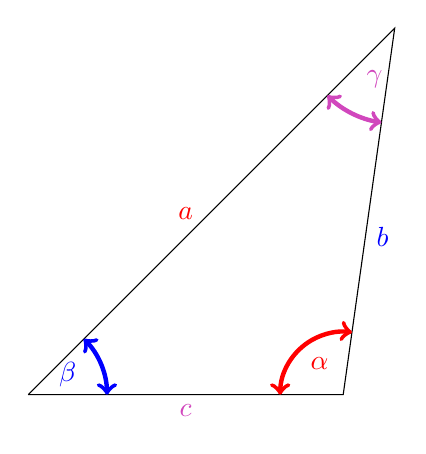
\begin{tikzpicture}[xscale=1,yscale=1]
    \draw[black] (0,0) -- (4,0) -- (4.654,4.654) -- (0,0);
    \node[blue] at (4.5,2) {$b$};
    \node[red] at (2,2.3) {$a$};
    \node[PINK, below] at (2,0) {$c$};
    \draw[blue, ultra thick, <->] (1,0) arc (0:45:1);
    \node[blue] at (0.5,0.25) {$\beta$};
    \draw[red, ultra thick, <->] (3.2,0) arc (180:82:0.8);
    \node[red] at (3.7,0.4) {$\alpha$};
    \draw[PINK, ultra thick, <->] (3.8,3.8) arc (225:262:1.207738);
    \node[PINK] at (4.4,4) {$\gamma$};
\end{tikzpicture}
\label{fig:math:law_of_sines}
\end{figure}
\end{flushleft}
\end{minipage}
~
\begin{minipage}{0.4\textwidth}
\begin{flushright}
\begin{gather*}
    \frac{\sin{\textcolor{red}{\alpha}}}{\textcolor{red}{a}} = \frac{\sin{\textcolor{blue}{\beta}}}{\textcolor{blue}{b}} = \frac{\sin{\textcolor{PINK}{\gamma}}}{\textcolor{PINK}{c}}
\end{gather*}
\end{flushright}
\end{minipage}

\newpage

\section{Calculus Primer}

\subsection{Differentiation}

\subsubsection{Differentiation from First Principles}

Consider a function $f$ that depends on only one variable $x$. Near any particular point the value of the function changes by an amount $\Delta f$, say, as $x$ changes by some amount $\Delta x$. We must let $\Delta x$ become infinitesimally small. We therefore define the first derivative of $f$ as
\begin{equation*}
    f'(x) \equiv \frac{d f}{dx} \equiv \lim\limits_{\Delta x \to 0} \frac{f(x + \Delta x) - f(x)}{\Delta x},
\end{equation*}

provided the limit exists.

\subsubsection{Some Derivatives}

Note that $a$ is a constant.

\begin{gather*}
    \frac{d}{dx} \left[ x^n \right] = nx^{n - 1}, \qquad \frac{d}{dx} \left[ e^{ax} \right] = ae^{ax}, \qquad \frac{d}{dx} \left[ \ln{ax} \right] = \frac{1}{x}, \\
    \frac{d}{dx} \left[ \sin{ax} \right] = a\cos{ax}, \frac{d}{dx} \left[ \cos{ax} \right] = -a\sin{ax}, \qquad \frac{d}{dx} \left[ \sec{ax} \right] = a\sec{ax}\tan{ax}, \\
    \frac{d}{dx} \left[ \tan{ax} \right] = a\sec^2{x}, \qquad \frac{d}{dx} \left[ \csc{ax} \right] = -a\csc{ax}\cot{ax}, \\
    \frac{d}{dx} \left[ \cot{ax} \right] = -a\csc^2{ax}, \qquad \frac{d}{dx} \left[ \sin^{-1}{\frac{x}{a}} \right] = \frac{1}{\sqrt{a^2 - x^2}}, \\
    \frac{d}{dx} \left[ \cos^{-1}{\frac{x}{a}} \right] = \frac{-1}{\sqrt{a^2 - x^2}}, \qquad \frac{d}{dx} \left[ \tan^{-1}{\frac{x}{a}} \right] = \frac{a}{a^2 + x^2}.
\end{gather*}

\subsection{Integration}

\subsubsection{Some Integrals}

Note that $a$ and $b$ are constants and the integrals that depend on $n$ are valid for $n \neq 1$. In the final two results $\left| x \right| \leqslant a$.

\begin{gather*}
    \int a\ dx = ax + C, \qquad \int ax^n dx = \frac{ax^{n + 1}}{n + 1} + C, \\
    \int e^{ax} dx = \frac{e^{ax}}{a} + C, \qquad \int \frac{a}{x}\ dx = a\ln{x} + C, \\
    \int a \cos{bx} dx = \frac{a\sin{bx}}{b} + C, \qquad \int a \sin{bx} dx = \frac{-a\cos{bx}}{b} + C, \\
    \int a\tan{bx}dx = \frac{-a\ln{\left( \cos{bx} \right)}}{b} + C, \qquad \int a\cos{bx}\sin^n{bx}dx = \frac{a\sin^{n + 1}{bx}}{b\left( n + 1 \right)} + C, \\
    \int \frac{a}{a^2 + x^2}dx = \tan^{-1}{\left( \frac{x}{a} \right)} + C, \qquad \int a\sin{bx}\cos^n{bx}dx = \frac{a\cos^{n + 1}{bx}}{b\left( n + 1 \right)} + C, \\
    \int \frac{-1}{\sqrt{a^2 - x^2}}dx = \cos^{-1}{\left( \frac{x}{a} \right)} + C, \qquad \int \frac{1}{\sqrt{a^2 - x^2}}dx = \sin^{-1}{\left( \frac{x}{a} \right)} + C
\end{gather*}

\subsubsection{Integration by Parts}

The product rule gives
\begin{equation*}
    \frac{d}{dx}(uv) = u\frac{dv}{dx} + \frac{du}{dx}v,
\end{equation*}

where $u$ and $v$ are functions of $x$. We integrate to find
\begin{equation*}
    uv = \int u \frac{dv}{dx}\ dx + \int \frac{du}{dx}v\ dx.
\end{equation*}

Rearranging into to the standard form for integration by parts gives
\begin{equation*}
    \int u \frac{dv}{dx}\ dx = uv - \int \frac{du}{dx}v\ dx.
\end{equation*}

\section{Polar Numbers and Hyperbolic Functions}

\subsection{Polar Representation of Complex Numbers}

Formally, a complex number is an ordered pair $\left( x, y \right)$, where $a, b \in \R$, but we write this as $x + iy$. The set of all complex numbers is denoted by $\mathbb{C}$:
\begin{equation*}
    \mathbb{C} = \left\{ x + iy : x, y \in \R \right\}.
\end{equation*}

Although considering an imaginary number as the sum of a real and an imaginary part is often useful, sometimes the \emph{polar representation} proves easier to manipulate. This makes use of the exponential function, which is defined by
\begin{equation*}
    e^z = \exp z \equiv 1 + z + \frac{z^2}{2!} + \frac{z^3}{3!} + \cdots.
\end{equation*}

It follows that for $z = i\theta$, $\theta$ real,
\begin{align*}
    e^{i\theta} &= 1 + i\theta - \frac{\theta^2}{2!} - \frac{i\theta^3}{3!} + \cdots \\
    &= 1 - \frac{\theta^2}{2!} + \frac{\theta^4}{4!} - \cdots + i \left( \theta - \frac{\theta^3}{3!} + \frac{\theta^5}{5!} \right)
\end{align*}

and hence that
\begin{equation*}
    e^{i\theta} = \cos{\theta} + i\sin{\theta}.
\end{equation*}

This last relationship is known as \emph{Euler's equation}. It also follows that
\begin{equation*}
    e^{in\theta} = \cos{n\theta} + i\sin{n\theta}
\end{equation*}

for all $n$. We deduce that
\begin{align*}
    re^{i\theta} &= r \left( \cos{\theta} + i\sin{\theta} \right) \\
    &= x + iy.
\end{align*}

Thus a complex number may be represented in polar form
\begin{equation*}
    z = re^{i\theta}.
\end{equation*}

\subsubsection{Hyperbolic Functions}

\section{Series}

\subsection{Taylor Series}
\begin{equation*}
    f(z) = f(a) + f'(a)(z - a) + \frac{f''(a)}{2!}(z - a)^2 + \frac{f'''(a)}{3!}(z - a)^3 + \cdots \qquad
\end{equation*}

\subsection{Some Series Expansions}

\begin{gather*}
    \sin{z} = z - \frac{z^3}{3!} + \frac{z^5}{5!} - \frac{z^7}{7!} + \cdots \qquad \text{for } -\infty < x < \infty, \\
    \sinh{z} = z + \frac{z^3}{3!} + \frac{z^5}{5!} + \frac{z^7}{7!} + \cdots \qquad \text{for } -\infty < x < \infty, \\
    \cos{z} = 1 - \frac{z^2}{2!} + \frac{z^4}{4!} - \frac{z^6}{6!} + \cdots \qquad \text{for } -\infty < x < \infty, \\
    \cosh{z} = 1 + \frac{z^2}{2!} + \frac{z^4}{4!} + \frac{z^6}{6!} + \cdots \qquad \text{for } -\infty < x < \infty, \\
    \tan^{-1}{z} = z - \frac{z^3}{3} + \frac{z^5}{5} - \frac{z^7}{7} + \cdots \qquad \text{for } -1 < z < 1, \\
    e^z = \exp{z} = 1 + z + \frac{z^2}{2!} + \frac{z^3}{3!} + \frac{z^4}{4!} + \cdots \qquad \text{for } -\infty < z < \infty \\
    \ln{(1 + z)} = z - \frac{z^2}{2} + \frac{z^3}{3} - \frac{z^4}{4} + \cdots \qquad \text{for } -1 < z \leqslant 1, \\
    \left( 1 + z \right)^n = 1 + nz + n \left( n - 1 \right) \frac{z^2}{2!} + n \left( n - 1 \right) \left( n - 2 \right) \frac{z^3}{3!} + \cdots \qquad \text{for } -\infty < z < \infty.
\end{gather*}

\section{Vector Algebra}

\subsection{Addition and subtraction of vectors}

Vector addition is both commutative, i.e.
\begin{equation*}
    \bm{a} + \bm{b} = \bm{b} + \bm{a},
\end{equation*}

and associative, e.g.
\begin{equation*}
    \bm{a} + \left( \bm{b} + \bm{c} \right) = \left( \bm{a} + \bm{b} \right) + \bm{c}.
\end{equation*}

The subtraction of two vectors is similar to their addition, that is,
\begin{equation*}
    \bm{a} - \bm{b} = a + \left( -\bm{b} \right),
\end{equation*}

where $-\bm{b}$ is a vector of equal magnitude but exactly opposite direction to vector $\bm{b}$. The subtraction of two equal vectors yields the zero vector, $\bm{0}$, which has zero magnitude and no associated direction.

\subsection{Multiplication by a scalar}

Multiplication of a vector by a scalar gives a vector in the same direction as the original but of a proportional magnitude. Multiplication by a scalar is associative, commutative, and distributive over addition. These properties are summarized below for arbitrary vectors $\bm{a}$ and $\bm{b}$ and arbitrary scalars $\lambda$ and $\mu$.
\begin{gather*}
    \left( \lambda \mu \right) \bm{a} = \lambda \left( \mu \bm{a} \right) = \mu \left( \lambda \bm{a} \right), \\
    \lambda \left( \bm{a} + \bm{b} \right) = \lambda \bm{a} + \lambda \bm{b}, \\
    \left( \lambda + \mu \right) \bm{a} = \lambda \bm{a} + \mu \bm{a}.
\end{gather*}

\subsection{Basis vectors and components}

Given any three vectors $\mathbf{e}_1$, $\mathbf{e}_2$, and $\mathbf{e}_3$, which do not all lie in a plane, it is possible, in a three-dimensional space, to write any other vector in terms of scalar multiples of them:
\begin{equation*}
    \bm{a} = a_1 \mathbf{e}_1 + a_2 \mathbf{e}_2 + a_3 \mathbf{e}_3.
\end{equation*}

The three vectors $\mathbf{e}_1$, $\mathbf{e}_2$, and $\mathbf{e}_3$ are said to \emph{form a basis} for $\R^3$. The three components $a_1$, $a_2$, and $a_3$ are called the \emph{components} of the vector $\bm{a}$ with respect to this basis.

A set of basis vectors must
\begin{enumerate}
    \item[(1)] have as many basis vectors as the number of dimensions (the basis must span the space) and
    \item[(2)] be \emph{linearly independent}. Formally, we demand
    \begin{equation*}
        c_1 \mathbf{e}_1 + c_2 \mathbf{e}_2 + c_3 \mathbf{e}_3 \neq \bm{0},
    \end{equation*}
    for any set of coefficients except $c_1 = c_2 = c_3 = 0$.
\end{enumerate}

If we wish to label points in space using a Cartesian coordinate system $(x,y,z)$, we may introduce the unit vectors $\ihat$, $\jhat$, and $\khat$, which point along the positive $x$-, $y$-, and $z$- axes respectively. A vector $\bm{a}$ may then be written as a sum of three vectors, each parallel to a different coordinate axis:
\begin{equation*}
    \bm{a} = a_x\ihat + a_y\jhat + a_z\khat.
\end{equation*}

We can consider the addition of vectors in terms of their components. The sum of two vectors $\bm{a}$ and $\bm{b}$ is found by simply adding their components, i.e.
\begin{align*}
    \bm{a} + \bm{b} &= a_x\ihat + a_y\jhat + a_z\khat + b_x\ihat + b_y\jhat + b_z\khat \\
    &= \left( a_x + b_x \right) \ihat + \left( a_y + b_y \right) \jhat + \left( a_z + b_z \right) \khat.
\end{align*}

\subsection{Magnitude of a vector}

The magnitude of a vector $\bm{a}$ is denoted $\left| \bm{a} \right|$ or simply $a$. In terms of its components in three-dimensional Cartesian coordinates, the magnitude of $\bm{a}$ is given by
\begin{equation*}
    a \equiv |\bm{a}| = \sqrt{a_x^2 + a_y^2 + a_z^2}.
\end{equation*}

A vector whose magnitude is unity is called a \emph{unit vector}. The unit vector in the direction $\bm{a}$ is usually notated $\hat{\bm{a}}$ and may be evaluated as
\begin{equation*}
    \hat{\bm{a}} = \frac{\bm{a}}{|\bm{a}|}.
\end{equation*}

\section{Vector Calculus}

\subsection{Position and Displacement Vectors}

The location of a point in three dimensions is given by its Cartesian coordinates $(x, y, z)$. The vector to that point from the origin is called the \emph{position vector}:
\begin{equation*}
    \bm{r} = x\ \ihat + y\ \jhat + z\ \khat.
\end{equation*}

\begin{figure}[H]
\captionsetup{width=0.8\textwidth,labelfont={color=black,bf},textfont={color=black}}
\centering
\tdplotsetmaincoords{70}{110}
\begin{tikzpicture}[scale=4,tdplot_main_coords]
    \draw[thick,->] (0,0,0) -- (1,0,0) node[anchor=north east]{$x$};
    \draw[thick,->] (0,0,0) -- (0,1,0) node[anchor=north west]{$y$};
    \draw[thick,->] (0,0,0) -- (0,0,1) node[anchor=south]{$z$};
    \coordinate (O) at (0,0,0);
    \tdplotsetcoord{R}{1.4}{50}{50};
    \tdplotsetcoord{RHAT}{1.6}{50}{50};
    
    \draw[ultra thick, blue, ->] (O) -- (R) node[blue, midway, above] {$\bm{r}$};
    
    \draw[thick, blue, ->] (R) -- (RHAT) node[blue, midway, above] {$\rhat$};
    
    \draw[blue, dashed] (Rx) -- (Rxy) node[blue, midway, below] {$y$};
    \draw[blue, dashed] (Ry) -- (Rxy) node[blue, midway, right] {$x$};
    \draw[blue, dashed] (R) -- (Rxy) node[blue, midway, right] {$z$};
    
\end{tikzpicture}
\label{fig:postion_vector}
\end{figure}

The magnitude of the position vector,
\begin{equation*}
    r = \sqrt{x^2 + y^2 + z^2},
\end{equation*}

is the distance from the origin, and
\begin{equation*}
    \rhat = \frac{\bm{r}}{r} = \frac{x\ \ihat + y\ \jhat + z\ \khat}{\sqrt{x^2 + y^2 + z^2}}
\end{equation*}

is a unit vector pointing radially outward. The \emph{infinitesimal displacement vector}, from $(x, y, z)$ to $(x + dx, y + dy, z + dz)$ is
\begin{equation*}
    d\bm{\ell} = dx\ \ihat + dy\ \jhat + dz\ \khat.
\end{equation*}

\subsection{Scalar and Vector Fields}

A field arises whenever a particular scalar or vector quantity is defined \emph{continuously} as a \emph{field} throughout some region of space (often the whole of space). The concept of a field is valid for spaces with an arbitrary number of dimensions, we will restrict ourselves to the familiar three-dimensional case.

A \emph{scalar} field $\phi(x,y,z)$ associates a scalar with each point in a region. For example, the electric potential $V(x,y,z)$ associates each point in space with some voltage.

A \emph{vector} field $\bm{a}(x,y,z)$ associates a vector with each point in a region. For example, the electric field $\bm{E}(x,y,z)$ associates each point in space with some electric field vector.

\subsection{Vector Operations}

The most important operations are those of finding the \emph{gradient} of a scalar field and the \emph{divergence} and \emph{curl} of a vector field. Central to all these operations is the vector operator $\nabla$, which is called the \emph{del} operator and in Cartesian coordinates is defined by
\begin{equation*}
    \nabla \equiv \ihat\ \frac{\partial}{\partial x} + \jhat\ \frac{\partial}{\partial y} + \khat\ \frac{\partial}{\partial z}.
\end{equation*}

\subsubsection{Gradient of a Scalar Field}

The \emph{gradient} of a scalar field $\phi(x, y, z)$ is defined by
\begin{equation*}
    \nabla \phi = \ihat\ \frac{\partial \phi}{\partial x} + \jhat\ \frac{\partial \phi}{\partial y} + \khat\ \frac{\partial \phi}{\partial z}.
\end{equation*}

For an infinitesimal vector displacement $d\bm{\ell}$, forming its scalar product with $\nabla \phi$, we obtain
\begin{align*}
    \nabla \phi \cdot d\bm{\ell} &= \left( \ihat\ \frac{\partial \phi}{\partial x} + \jhat\ \frac{\partial \phi}{\partial y} + \khat\ \frac{\partial \phi}{\partial z} \right) \left( \ihat\ dx + \jhat\ dy + \khat\ dz \right) \\
    &= \frac{\partial \phi}{\partial x} dx + \frac{\partial \phi}{\partial y} dy + \frac{\partial \phi}{\partial z} dz \\
    &= d\phi,
\end{align*}

which is the infinitesimal change in $\phi$ in going from position $\bm{r}$ to $\bm{r} + d\bm{\ell}$. In general, the rate of change of $\phi$ with respect to the distance $s$ in a particular direction $\bm{a}$ is given by
\begin{equation*}
    \frac{d\phi}{ds} = \nabla \phi \cdot \hat{\bm{a}}
\end{equation*}

and is called the directional derivative. Since $\hat{\bm{a}}$ is a unit vector we have
\begin{equation*}
    \frac{d\phi}{ds} = \left| \nabla \phi \right| \cos{\theta}
\end{equation*}

where $\theta$ si the angle between $\hat{\bm{a}}$ and $\nabla \phi$. Clearly, the gradient $\nabla \phi$ points in the direction of maximum increase of the function $\phi$ (consider $\theta = 0$). Moreover, the magnitude $\left| \nabla \phi \right|$ gives the slope (rate of increase) along this maximal direction. Similarly, the largest rate of decrease of $\phi$ is $-\left| \nabla \phi \right|$ in the direction of $-\nabla \phi$.

\subsubsection{Divergence of a Vector Field}

The \emph{divergence} of a vector field $\bm{a}(x, y, z)$ is defined by
\begin{equation*}
    \nabla \cdot \bm{a} = \frac{\partial a_x}{\partial x} + \frac{\partial a_y}{\partial y} + \frac{\partial a_z}{\partial z},
\end{equation*}

where $a_x$, $a_y$, and $a_z$ are the $x$-, $y$-, and $z$- components of $\bm{a}$. Clearly, $\nabla \cdot \bm{a}$ is a scalar field. The divergence can be considered as a quantitative measure of how much a vector field diverges (spreads out) or converges at a particular point.

Now if some vector field $\bm{a}$ is itself derived from a scalar field via $\bm{a} = \nabla \phi$ then $\nabla \cdot \bm{a}$ has the form $\nabla \cdot \nabla \phi$ or, as it is usually written, $\nabla^2 \phi$, where $\nabla^2$ (del squared) is the scalar differential operator
\begin{equation*}
    \nabla^2 \equiv \frac{\partial^2}{\partial x^2} + \frac{\partial^2}{\partial y^2} + \frac{\partial^2}{\partial z^2}.
\end{equation*}

Note that $\nabla^2 \phi$ is called the \emph{Laplacian} of $\phi$.


\subsubsection{Curl of a Vector Field}

The \emph{curl} of a vector field $\bm{a}(x, y, z)$ is defined by
\begin{equation*}
    \nabla \times \bm{a} = \left( \frac{\partial a_z}{\partial y} - \frac{\partial a_y}{\partial z} \right)\ \ihat + \left( \frac{\partial a_x}{\partial z} - \frac{\partial a_z}{\partial x} \right)\ \jhat + \left( \frac{\partial a_y}{\partial x} - \frac{\partial a_x}{\partial y} \right)\ \khat,
\end{equation*}

where $a_x$, $a_y$, and $a_z$ are the $x$-, $y$- and $z$- components of $\bm{a}$. The RHS can be written in a more memorable form as a determinant:
\begin{equation*}
    \nabla \times \bm{a} = \begin{vmatrix} \ihat & \jhat & \khat \\ \partial/\partial x & \partial/\partial y & \partial/\partial z \\ a_x & a_y & a_z \end{vmatrix}.
\end{equation*}

Clearly, $\nabla \times \bm{a}$ is a vector field.

\subsection{Cylindrical Coordinates}

\subsection{Spherical Coordinates}

\section{Line, Surface, and Volume Integrals}

\section{The Dirac Delta Function}

\section{}

\end{document}
